\documentclass[12pt]{article}

% Packages
\usepackage[margin=1in]{geometry}
\usepackage{amsmath,amssymb,amsthm}
\usepackage{enumitem}
\usepackage{hyperref}
\usepackage{xcolor}
\usepackage{import}
\usepackage{xifthen}
\usepackage{pdfpages}
\usepackage{transparent}
\usepackage{listings}
\usepackage{tikz}
\usepackage{physics}
\usepackage{siunitx}
\usepackage{booktabs}
\usepackage{cancel}
  \usetikzlibrary{calc,patterns,arrows.meta,decorations.markings}


\DeclareMathOperator{\Log}{Log}
\DeclareMathOperator{\Arg}{Arg}

\lstset{
    breaklines=true,         % Enable line wrapping
    breakatwhitespace=false, % Wrap lines even if there's no whitespace
    basicstyle=\ttfamily,    % Use monospaced font
    frame=single,            % Add a frame around the code
    columns=fullflexible,    % Better handling of variable-width fonts
}

\newcommand{\incfig}[1]{%
    \def\svgwidth{\columnwidth}
    \import{./Figures/}{#1.pdf_tex}
}
\theoremstyle{definition} % This style uses normal (non-italicized) text
\newtheorem{solution}{Solution}
\newtheorem{proposition}{Proposition}
\newtheorem{problem}{Problem}
\newtheorem{lemma}{Lemma}
\newtheorem{theorem}{Theorem}
\newtheorem{remark}{Remark}
\newtheorem{note}{Note}
\newtheorem{definition}{Definition}
\newtheorem{example}{Example}
\newtheorem{corollary}{Corollary}
\theoremstyle{plain} % Restore the default style for other theorem environments
%

% Theorem-like environments
% Title information
\title{Mathematics of Guitar Strings}
\author{Jerich Lee}
\date{\today}

\begin{document}

\maketitle
The mechanical analysis for the rotary spring mechanism begins with the free body diagram
of the initial state of the guitar, as shown in Figure 12, and the final state of the guitar, as shown in
Figure 13. The free body diagram gives initial length as the sum of $a+b$ , where $a$ is the length
between the boundaries of the string, which the user plays, and $b$ is the length between the
boundary point of $a$ and the guitar string tuning key.

\begin{figure}[htbp]
  \centering
  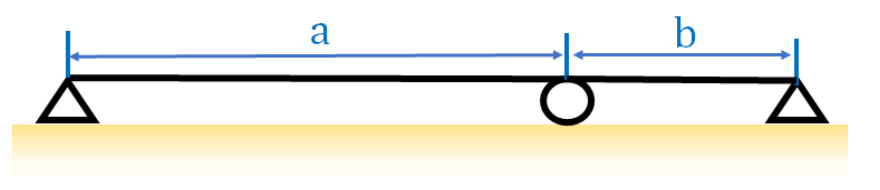
\includegraphics[width=0.8\textwidth]{classes/Mathematics-of-Guitar-Strings/06-10/fgs/fig12.png}
  \caption{Free Body Diagram of Initial State}
  \label{fig:}
\end{figure}

\begin{figure}[htbp]
  \centering
  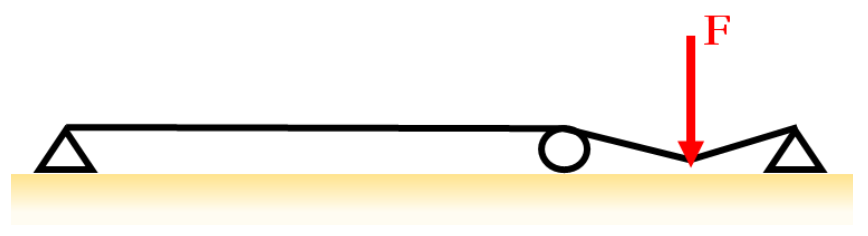
\includegraphics[width=0.8\textwidth]{classes/Mathematics-of-Guitar-Strings/06-10/fgs/fig13.png}
  \caption{Free Body Diagram of Deformed State}
  \label{fig:}
\end{figure}

% ----------------------------------------------------------------
%  Text plus numbered equations (1)–(6)
%  – uses equation/align* for \tag{}; inline symbols in $$ ... $$
% ----------------------------------------------------------------

The equation that relates frequency to the tension of a guitar string is
the vibrating–string equation shown in \textbf{Equation~1}:

\begin{equation}
  f \;=\; \frac{1}{2L}\sqrt{\frac{T}{\rho_L}}
  \tag{1}
\end{equation}

By performing a Taylor-series expansion of Equation 1 with respect to
tension, the partial derivative of frequency with respect to tension is

\begin{equation}
  \frac{\partial f}{\partial T}
    \;=\;
  \frac{1}{4L\sqrt{T\rho_L}}
  \tag{2}
\end{equation}

Simple algebraic manipulation of Equation 1 yields

\begin{equation}
  \frac{f_0}{T_0}
    \;=\;
  \frac{1}{2L\sqrt{T\rho_L}}
  \tag{3}
\end{equation}

Using a first-order Taylor expansion, the frequency after a small change
in tension $\Delta T$ becomes

\begin{equation}
  f \;=\; f_0 \;+\;
       \frac{\partial f}{\partial T}\,\Delta T
  \tag{4}
\end{equation}

Accordingly, the change in frequency is

\begin{equation}
  \Delta f
    \;=\;
  \frac{\partial f}{\partial T}\,\Delta T
  \tag{5}
\end{equation}

Finally, substituting Equation 3 into Equation 2 shows that

\begin{equation}
  \frac{\partial f}{\partial T}
    \;=\;
  \tfrac12\,\frac{f_0}{T_0}
  \tag{6}
\end{equation}

% ----------------------------------------------------------------
%  Derivations leading to Equations (7)–(13) with surrounding text
% ----------------------------------------------------------------

By plugging Equation~(6) into Equation~(5), we obtain

\begin{equation}
  \Delta f \;=\; \frac{1}{2}\,\frac{f_0}{T_0}\,\Delta T
  \tag{7}
\end{equation}

Re-arranging Equation (7) gives the change in tension in terms of the
initial tension $$T_0$$, initial frequency $$f_0$$, and the desired
frequency shift $$\Delta f$$:

\begin{equation}
  \Delta T \;=\; 2T_0\,\frac{\Delta f}{f_0}
  \tag{8}
\end{equation}

---

\paragraph*{Constitutive relations.}
Using the definition of normal stress $$\sigma$$ as force divided by
cross-sectional area and the engineering strain $$\epsilon$$ as the
fractional change in length,

\begin{equation}
  \sigma \;=\; \frac{F}{A}
  \tag{9}
\end{equation}

\begin{equation}
  \epsilon \;=\; \frac{L - L_0}{L_0},
  \tag{10}
\end{equation}

and assuming linear elasticity (Hooke’s law)

\begin{equation}
  \sigma \;=\; E\,\epsilon,
  \tag{11}
\end{equation}

we can combine (9)–(11) to obtain

\begin{equation}
  \frac{F}{A}
    \;=\;
  E\,\frac{L - L_0}{L_0}.
  \tag{12}
\end{equation}

---

\paragraph*{Axial string displacement.}
The axial displacement of the string is simply the difference between the
current length $$L$$ and the original length $$L_0$$:

\begin{equation}
  \delta \;=\; L - L_0.
  \tag{13}
\end{equation}

Thus, once $$\delta$$ is determined from the geometric relations in the
next section, Equations (8) and (12) can be used to calculate the tension
increment $$\Delta T$$ and the corresponding axial force $$F$$ required to
achieve the target frequency shift.

\begin{figure}[htbp]
  \centering
  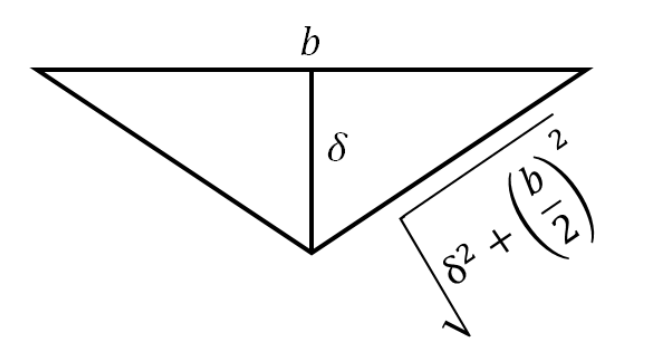
\includegraphics[width=0.8\textwidth]{classes/Mathematics-of-Guitar-Strings/06-10/fgs/fig14.png}
  \caption{Free Body Diagram of Deformed Region}
  \label{fig:}
\end{figure}

% ----------------------------------------------------------------
%  Geometry: initial length, deflected length, strain, displacement
%  (Equations 14–17 with explanatory text; inline math uses $ $)
% ----------------------------------------------------------------

\begin{equation}
  L_0 \;=\; a + b
  \tag{14}
\end{equation}

\begin{equation}
  L \;=\; a + 2\sqrt{\delta^{2} + \Bigl(\dfrac{b}{2}\Bigr)^{2}}
  \tag{15}
\end{equation}

Equation\,14 and Equation\,15 can be substituted into Hooke’s-law
relation~(11) to obtain the strain of the string in terms of the vertical
deflection $\delta$ and the baseline lengths $a$ and $b$:

\begin{equation}
  \frac{L - L_0}{L_0}
    \;=\;
  \frac{\,2\sqrt{\delta^{2} + \bigl(\dfrac{b}{2}\bigr)^{2}}\; -\; b}{\,a + b}
  \tag{16}
\end{equation}

Solving Equation 16 for the vertical displacement $\delta$ yields

\begin{equation}
  \delta
    \;=\;
  \sqrt{
    \Bigl(
      \frac{\Delta T\,(a+b)}{2(EA)_{\!\mathrm{eff}}}
      + \frac{b}{2}
    \Bigr)^{2}
    \;-\;
    \Bigl(\frac{b}{2}\Bigr)^{2}}
  \tag{17}
\end{equation}

The value of $\delta$ in Equation 17 provides the \emph{horizontal
displacement} that the user’s foot must apply to the pedal so the string
reaches the target frequency consistently.  All quantities on the right
side are either measured ($a$, $b$), experimentally characterised
[$T_0$, $(EA)_{\!\text{eff}}$], or specified by the musician
($\Delta f = f - f_0$).

The force applied when the string displaces by $$\delta$$ is obtained
from the free-body diagram in Figure 15.  
By resolving the component forces along the $$y$$-axis, one arrives at
Equations (18) and (19).

\begin{figure}[htbp]
  \centering
  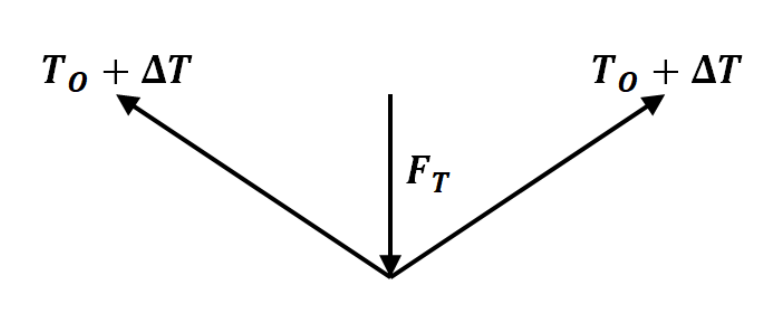
\includegraphics[width=0.8\textwidth]{classes/Mathematics-of-Guitar-Strings/06-10/fgs/fig15.png}
  \caption{Free Body Diagram of Forces at Deformed Region}
  \label{fig:}
\end{figure}

\begin{equation}
  \sum F_y \;=\; 0
  \;=\;
  2\bigl(T_0+\Delta T\bigr)
  \frac{\delta}{\sqrt{\delta^{2}+b^{2}/4}}
  \tag{18}
\end{equation}

\begin{equation}
  F_T
  \;=\;
  2\bigl(T_0+\Delta T\bigr)\,
  \frac{\delta}{\sqrt{\delta^{2}+\bigl(\frac{b}{2}\bigr)^{2}}}
  \tag{19}
\end{equation}

To solve for the vertical displacement of the string in \textbf{Equation 17}
and for the applied force required in \textbf{Equation 18}, the constants
$$a$$, $$b$$, $$f_0$$, $$\Delta f$$, $$T_0$$ and $$(EA)_{\text{eff}}$$
must be known.  The values $$a$$ and $$b$$ are obtained by measuring the
distance between the string boundaries and the distance from the boundary
point at $$a$$ to the guitar’s tuning key, respectively.  The initial
frequency $$f_0$$ and the desired frequency change $$\Delta f$$ are found
from the difference between the initial note~G$$\sharp$$3 and the final
note~A3.  Finally, the initial tension $$T_0$$ and the effective axial
stiffness $$(EA)_{\text{eff}}$$ are determined experimentally.
Table 1 lists these values.

% ------------------------------------------------------------
%  Table 1 – Constants for the Guitar String
% ------------------------------------------------------------
\begin{table}[ht]
  \centering
  \caption*{Table 1.\;Constants for Guitar String}
  \begin{tabular}{|l|c|}
  \hline
  \textbf{Constant} & \textbf{Value} \\ \hline
  $a$               & 22.50\,in \\ \hline
  $b$               & 7.374\,in \\ \hline
  $f_0$             & 207.7\,Hz \\ \hline
  $T_0$             & 29.5983\,lb \\ \hline
  $\Delta f$        & 12.460\,Hz \\ \hline
  $(EA)_{\text{eff}}$ & 4638\,lb \\ \hline
  \end{tabular}
  \end{table}
  
  After the constants are known, they are substituted into
  Equation (8), Equation (17), and Equation (18) to obtain
  the values of the functions $\Delta T$, $\delta$, and $F_T$,
  summarised in Table 2.
  
  % ------------------------------------------------------------
  %  Table 2 – Calculated Quantities
  % ------------------------------------------------------------
  \begin{table}[ht]
  \centering
  \caption*{Table 2.\;Values of Interest for Guitar String}
  \begin{tabular}{|l|c|}
  \hline
  \textbf{Function} & \textbf{Value} \\ \hline
  $\Delta T$ & 3.55\,lb \\ \hline
  $\delta$   & 0.29\,in \\ \hline
  $F_T$      & 5.21\,lb \\ \hline
  \end{tabular}
  \end{table}
  
  Using these solved values, the required change in string length
  $\delta = 0.29$\,in produces the pitch A3, and the force required to
  achieve this displacement is $F_T = 5.21$\,lb.  Because the player will
  apply the load via a foot pedal rather than directly at the head-stock,
  a static analysis of the pedal is needed.  Of particular interest are
  (i)~the angular displacement needed to produce $\delta$ and (ii)~the
  force required at the pedal.  Figures 16 and 17 illustrate the pedal
  mechanism.  A stop pin fixes the pedal at an exact angular position,
  ensuring consistent notes.  The design task is therefore to determine
  the pin height $h$ (see the free-body diagram in Figure 18) as a
  function of the initial and final frequencies.

  \begin{figure}[htbp]
    \centering
    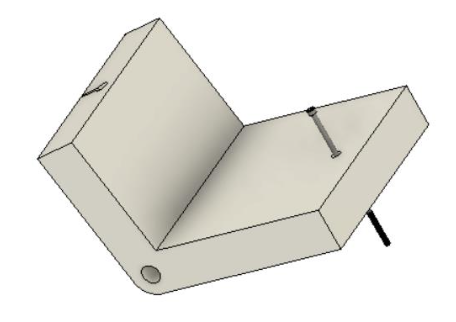
\includegraphics[width=0.8\textwidth]{classes/Mathematics-of-Guitar-Strings/06-10/fgs/fig16.png}
    \caption{Side Angle View of Pedal}
    \label{fig:}
  \end{figure}
  \begin{figure}[htbp]
    \centering
    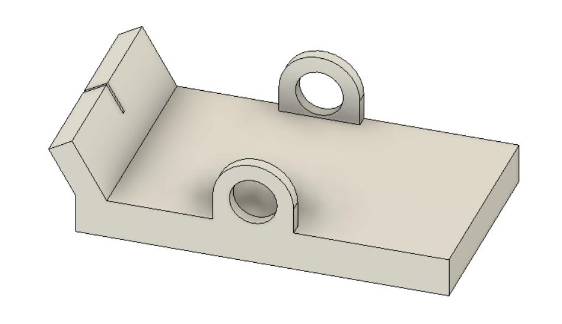
\includegraphics[width=0.8\textwidth]{classes/Mathematics-of-Guitar-Strings/06-10/fgs/fig17.png}
    \caption{Side Angle View of Foot Pedal Base}
    \label{fig:}
  \end{figure}

  \begin{figure}[htbp]
    \centering
    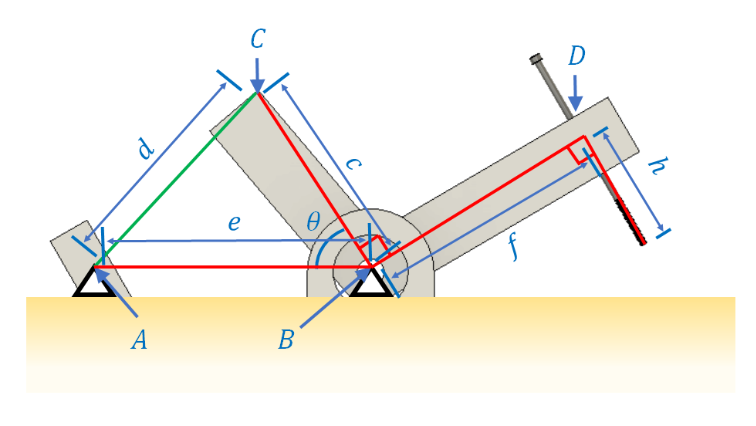
\includegraphics[width=0.8\textwidth]{classes/Mathematics-of-Guitar-Strings/06-10/fgs/fig18.png}
    \caption{Free Body Diagram of Initial State of Foot Pedal}
    \label{fig:}
  \end{figure}

  The constant dimensions of the foot pedal are listed in Table 3.
The green line $d$ represents the string segment that runs from
pin $C$ to pin $A$.
An external force is applied at point $D$, causing the pedal to rotate
about pin $B$.
This rotation lengthens~$d$; our goal is to choose the pedal’s angular
displacement so that $d$ increases by precisely the vertical string
deflection $\delta$ required to reach the target frequency A3.
That same rotation fixes the pin height $h$ that will hold the pedal at
the desired angle when the player presses down, because the reaction
forces at the base keep the angle stable.
Determining $h$ therefore begins with computing the length~$d$ via the
Law of Cosines (Figure 19).

% ------------------------------------------------------------
%  Table 3 – Constants for Foot Pedal (no tabularx)
% ------------------------------------------------------------
\begin{table}[ht]
\centering
\caption*{Table 3.\;Constants for Foot Pedal}
\begin{tabular}{|l|c|}
\hline
\textbf{Constant} & \textbf{Value} \\ \hline
$c$ & 2.50\,in \\ \hline
$e$ & 3.10\,in \\ \hline
$f$ & 3.40\,in \\ \hline
$\theta$ & 60$^\circ$ \\ \hline
\end{tabular}
\end{table}

\begin{figure}[htbp]
  \centering
  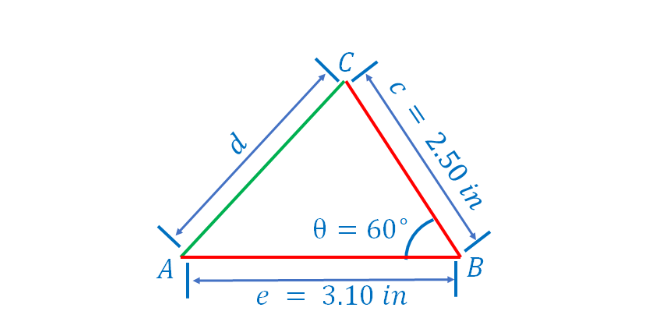
\includegraphics[width=0.8\textwidth]{classes/Mathematics-of-Guitar-Strings/06-10/fgs/fig19.png}
  \caption{Free Body Diagram of Initial State of Triangle ABC}
  \label{fig:}
\end{figure}

The Law of Cosines gives the original length $d$ of the green segment:

\begin{equation}
  d^{2} \;=\; e^{2} + c^{2} - 2ec\cos\theta
  \tag{20}
\end{equation}

\begin{equation}
  d \;=\; \sqrt{e^{2} + c^{2} - 2ec\cos\theta}
  \tag{21}
\end{equation}

Once $d$ is known, the new pedal angle $\gamma$ is obtained with a second
application of the Law of Cosines in Equations 22 and 23 (see the free-body
diagram in Figure 20).  Here $\gamma$ is the post-actuation angle
$\angle ABC$ that produces a total string displacement of
$d + \delta$ inches.

\begin{figure}[htbp]
  \centering
  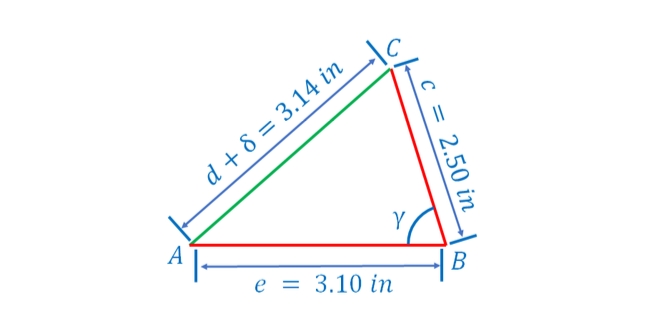
\includegraphics[width=0.8\textwidth]{classes/Mathematics-of-Guitar-Strings/06-10/fgs/fig20.png}
  \caption{Free Body Diagram of Actuated State of Triangle ABC}
  \label{fig:}
\end{figure}

\begin{equation}
  (d+\delta)^{2}
  \;=\;
  c^{2} + e^{2} - 2ce\cos\gamma
  \tag{22}
\end{equation}

\begin{equation}
  \gamma
  \;=\;
  \arccos\!\left(
    \frac{c^{2}+e^{2}-(d+\delta)^{2}}{2ce}
  \right)
  \tag{23}
\end{equation}

After $\gamma$ is known, its complement
$\alpha = \angle DBE$ (see Figure 21) is

\begin{equation}
  \alpha \;=\; 90^{\circ} - \gamma
  \tag{24}
\end{equation}

The angle $\alpha$ is then used to determine the nail height $h$ in
Equation 21.

\begin{figure}[htbp]
  \centering
  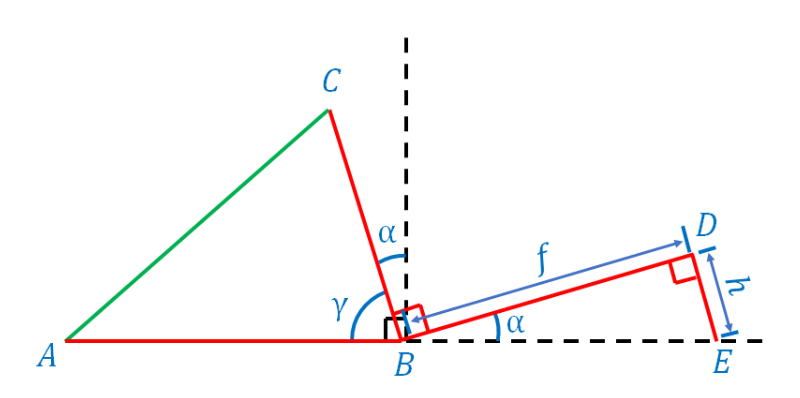
\includegraphics[width=0.8\textwidth]{classes/Mathematics-of-Guitar-Strings/06-10/fgs/fig21.png}
  \caption{Free Body Diagram of Actuated State of Foot Pedal}
  \label{fig:}
\end{figure}

\begin{equation}
  \tan\alpha \;=\; \frac{h}{f}
  \tag{24}
\end{equation}

\begin{equation}
  h \;=\; f\,\tan\alpha
  \tag{25}
\end{equation}

The constant dimensions of the foot pedal are substituted into
Equation (21), Equation (23), and Equation (25) to obtain the
quantities listed in Table 4.

% ------------------------------------------------------------
%  Table 4 – Values of Interest for Foot Pedal
% ------------------------------------------------------------
\begin{table}[ht]
\centering
\caption*{Table 4.\;Values of Interest for Foot Pedal}
\begin{tabular}{|l|c|}
\hline
\textbf{Function} & \textbf{Value} \\ \hline
$d$   & 2.85\,in \\ \hline
$\alpha$ & 22.82$^\circ$ \\ \hline
$h$   & 1.43\,in \\ \hline
\end{tabular}
\end{table}

Table 4 shows the exact length $h$ required for the nail at the end of the
pedal to ensure the final string frequency is 220.16 Hz (note A3).
To determine the force applied to the pedal to achieve this frequency,
the angle $\beta$ must be obtained from the Law of Cosines, as illustrated
in Figure 22 and expressed in Equation 27.

\begin{figure}[htbp]
  \centering
  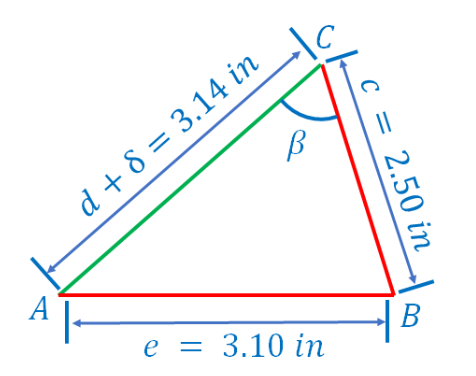
\includegraphics[width=0.8\textwidth]{classes/Mathematics-of-Guitar-Strings/06-10/fgs/fig22.png}
  \caption{Free Body Diagram of Triangle ABC}
  \label{fig:}
\end{figure}

\begin{equation}
  e^{2}
  \;=\;
  c^{2} + (d+\delta)^{2} - 2c(d+\delta)\cos\beta
  \tag{26}
\end{equation}

\begin{equation}
  \beta \;=\;
  \arccos\!\left(
    \frac{c^{2} + (d+\delta)^{2} - e^{2}}{\,2c(d+\delta)}
  \right)
  \tag{27}
\end{equation}

The force that must be applied at the end of the pedal to realize this
geometry is obtained from the free-body diagram in Figure 23 and is
expressed in Equation 28 and Equation 29.

\begin{figure}[htbp]
  \centering
  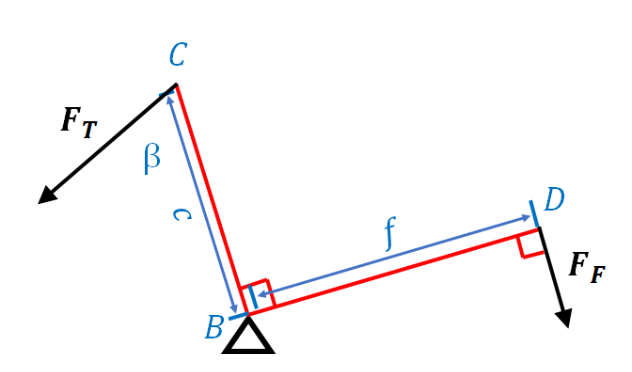
\includegraphics[width=0.8\textwidth]{classes/Mathematics-of-Guitar-Strings/06-10/fgs/fig23.png}
  \caption{Free Body Diagram of Forces on Pedal}
  \label{fig:}
\end{figure}

\begin{equation}
  \sum M_B = 0
  \;=\;
  cF_T\sin\beta \;-\; f\,F_F
  \tag{28}
\end{equation}

\begin{equation}
  F_F
  \;=\;
  \frac{cF_T\sin\beta}{f}
  \tag{29}
\end{equation}

Table 5 summarises the solved values of $\beta$ and the pedal force $F_F$.
The required force on the pedal to lower the string to note A3 is
$F_F = 3.49$\,lb.

% ------------------------------------------------------------
%  Table 5 – Forces for the Foot Pedal
% ------------------------------------------------------------
\begin{table}[ht]
\centering
\caption*{Table 5.\;Values of Interest for Forces on Foot Pedal}
\begin{tabular}{|l|c|}
\hline
\textbf{Function} & \textbf{Value} \\ \hline
$\beta$ & 65.56$^\circ$ \\ \hline
$F_F$   & 3.49\,lb \\ \hline
\end{tabular}
\end{table}

The force applied at the pedal is therefore smaller than the direct force
needed at the head-stock: the pedal requires only $3.49$\,lb whereas the
string tension change demands $F_T = 5.21$\,lb.  
The resulting mechanical advantage—because the pedal acts as a class-I
lever—is

\begin{equation}
  MA \;=\; \frac{F_T}{F_F} \;=\; 1.49
  \tag{30}
\end{equation}
\end{document}
